\documentclass{article}
\usepackage[utf8]{inputenc}

\title{Deep Residual Learning for Image Recognition}
\author{}
\date{}

\usepackage{natbib}
\usepackage{graphicx}
\usepackage{amsmath}
\usepackage[left=2.5cm,right=2.5cm,top=1cm,bottom=1.25cm]{geometry}
\usepackage{hyperref}
\usepackage{float}
\usepackage[export]{adjustbox}
\usepackage{sidecap}
\hypersetup{colorlinks=true,urlcolor=blue}
\pagenumbering{gobble}

\begin{document}

\maketitle

\section*{Link}
\href{https://arxiv.org/abs/1512.03385}{arxiv} 

\section*{Summary}
\begin{itemize}
    \item When deeper networks are able to start converging, a degradation problem has been exposed: with the network depth increasing, accuracy gets saturated and then degrades rapidly. Unexpectedly, such degradation is not caused by overfitting, and adding more layers to a suitably deep model leads to higher \textbf{training error}(not just validation error). This suggests that not all systems are similarly easy to optimize. Let us consider a shallower architecture and its deeper counterpart that adds more layers onto it. There exists a solution by construction to the deeper model: the added layers are identity mapping, and the other layers are copied from the learned shallower model. The existence of this constructed solution indicates that a deeper model should produce no higher training error than its shallower counterpart. 
    \item Instead of hoping each few stacked layers directly fit a desired underlying mapping, we explicitly let these layers fit a residual mapping. Formally, denoting the desired underlying mapping as $H(x)$, we let the stacked nonlinear layers fit another mapping of $F(x) := H(x) - x$. The original mapping is recast into $F(x) + x$. We hypothesize that it is easier to optimize the residual mapping than to optimize the original, unreferenced mapping. To the extreme, if an identity mapping were optimal, it would be easier to push the residual to zero than to fit an identity mapping by a stack of nonlinear layers. This formulation is realized by the shortcut connections as seen in the following figure.
    \begin{figure}[H]
        \centering
        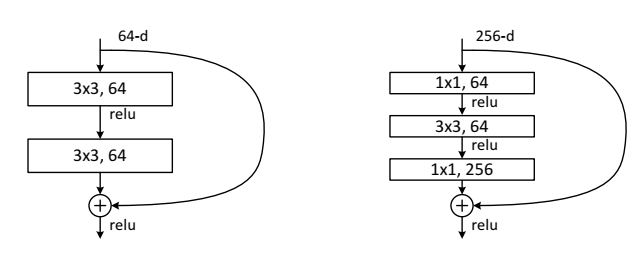
\includegraphics[scale=0.75]{residual_block.png}
        \caption{Residual block}
        \label{fig:Figure 1}
    \end{figure}
    \item When adding shortcut connection between input and output that have same dimensions we use identity mapping i.e.,
    \begin{equation*}
        y = F(x, {W_i}) + x 
    \end{equation*}
    When dimensions increase we try two option
    \begin{enumerate}
        \item The shortcut still performs identity mapping, with extra zero entries padded for increasing dimensions. This option introduces no extra parameter.
        \item We can perform a linear projection $W_s$ by the shortcut connections to match the dimensions:
        \begin{equation*}
            y = F(x, {W_i}) + W_s x 
        \end{equation*}
        This adds extra para mater. We could also do this for matching dimensions but it didn't show significant gain in performance.
    \end{enumerate}
    \item For training deeper nets they use a bottleneck structure(Figure 1. right) where they use a stack of three layers instead of two. 
    \item This ResNet approach doesn't show training accuracy degradation like just linearly stacking layer does as evident in Figure 2.
    \begin{figure}[H]
        \centering
        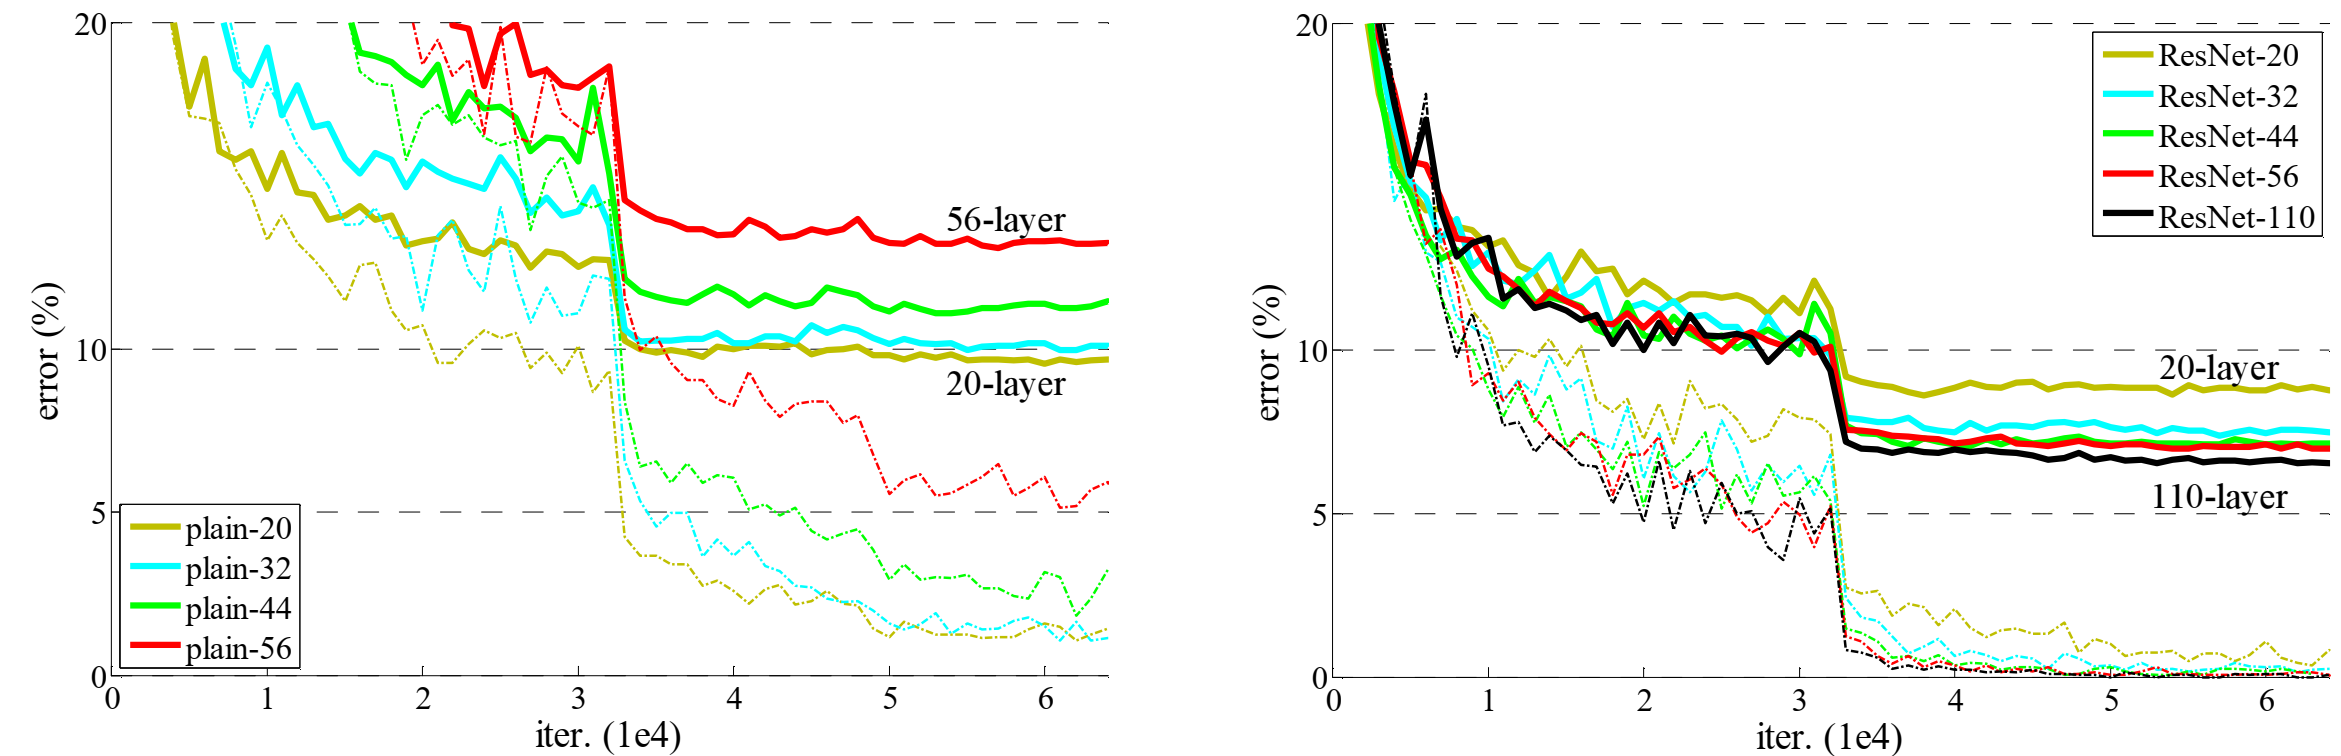
\includegraphics[scale=0.26]{cifar10_results.png}
        \caption{Training on CIFAR-10. Dashed lines denote training error, and bold lines denote testing error.}
        \label{fig:Figure 2}
    \end{figure}
    \item An ensemble of these residual nets achieves 3.57\% error on the ImageNet test set. This result won the 1st place on the ILSVRC 2015 classification task. Their ResNet based approach also won the 1st places on the tasks of ImageNet detection, ImageNet localization, COCO detection, and COCO segmentation in 2015.

\end{itemize}

\end{document}
